\scanpage{13}
\uline{Ex} $C=\operatorname{Ens}(\pi')$
\margin{\textcircled{2}}

\diagram{\begin{tikzcd}[ampersand replacement=\&,row sep=large]
\underset{\substack{\tikz[baseline=-.3ex]\draw (0,.17)..controls(-.08,.03)and(-.05,-.06)..(.03,-.09);\text{commutant}\\\text{aux }\varinjlim}}{\underline{\operatorname{Hom}}_!}\bigl(\operatorname{Ens}(\pi),\operatorname{Ens}(\pi')\bigr)\arrow[r,phantom,"\simeq"]\&{}_{\pi'}\operatorname{Ens}_\pi\arrow[d,phantom,"\rotatebox{90}{$\in$}"]\\
\&{}_{\pi'}X_\pi
\end{tikzcd}}


\diagram{\begin{tikzcd}[ampersand replacement=\&,column sep=large]
X\arrow[d,leftrightarrow]\&\operatorname{Ens}(\pi)\arrow[d,phantom,"\rotatebox{90}{$\in$}"]\\
F:\&E\arrow[r,maps to]\&X\times_\pi E
\end{tikzcd}}

\uline{Proposition} Pour que $F$ soit exact à gauche,
il f. et s. que $X$ soit un $\pi$-torseur à droite.
\figure{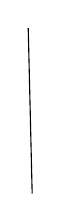
\begin{tikzpicture}\draw (0,0)--(.05,-2.1);\end{tikzpicture}}

$X$ torseur sous $\pi$
\[
{}^X\pi\overset{\mathrm{df}}=X\times_\pi\operatorname{int}(\pi)=\operatorname{Aut}_\pi(X)
\]
\[
\pi'\longrightarrow\operatorname{Aut}_\pi(X)
\]

\uline{Corollaire} Pour que $F$ soit équivalence, il f et s que
$\pi'\xrightarrow{\sim}\operatorname{Aut}_\pi(X)$, i.e. que $X$ soit un
bitorseur sous $\pi',\pi$; donc

\diagram{\begin{tikzcd}[ampersand replacement=\&,column sep=large,row sep=large]
\underline{\operatorname{Équiv}}\bigl(\operatorname{Ens}(\pi),\operatorname{Ens}(\pi')\bigr)\arrow[r,phantom,"\approxeq"]\arrow[d,"\wr"',"u\longmapsto u^{[-1]}"]\&\operatorname{BiL}(\pi',\pi^{\unsure{3|*}})\arrow[d,"u"]\\
\underline{\operatorname{Equiv}}\bigl(\operatorname{Ens}(\pi'),\operatorname{Ens}(\pi)\bigr)\arrow[r,"\approx"]\&\operatorname{Bit}(\pi,\pi')
\end{tikzcd}}

\mspage{12}
